\chapter{Do Calculus}\label{ch-do-calc}


The Do Calculus and associated ideas were
invented by
Judea Pearl and collaborators.
This chapter is 
based on Judea Pearl's
books (see Chapter \ref{ch0-nav-pearl}).


When
doing
Do Calculus,
it is 
convenient
to separate
the nodes
of a bnet
into
2  types:
{\bf observed},
and {\bf hidden (i.e., unobserved, latent,
unmeasured, non-visible)},
depending
on
whether data
describing
the
state 
of that
node
is available  (i.e., measured) or not.
In this chapter, every
hidden node will 
be indicated 
in a bnet
diagram by
either: (1)
enclosing
its random variable
in a dashed circle or
(2) making
the arrows
coming
out of it
dashed.
Accordingly, 
the 
3 diagrams 
in
Fig.\ref{fig-hidden-dashes}
all mean the same thing.

A {\bf confounder node} $\rvc$
for nodes $\rvx$ and $\rvy$
is a root node
with arrows
pointing
from it to
both
$\rvx$ and $\rvy$.
Thus, $\rvc$ acts as a {\bf common cause}
of $\rvx$ and $\rvy$.
In general, confounders
can be either observed
or hidden nodes.
The word ``confounder" itself
just means that it confuses
the analysis.
It says nothing about
whether it is hidden or not.
The node
$\rvc$
in Fig.\ref{fig-hidden-dashes})
is a {\bf hidden confounder}.

\begin{figure}[h!]
$$\xymatrix{
&*++[F-o]{\rvc}\ar[dl]\ar[dr]
\\
\rvx\ar[rr]&&\rvy
}
\;\;\;
\xymatrix{
\rvx\ar@{-->}@{<-->}@/^2pc/[rr]
\ar[rr]&&\rvy
}
\;\;\;
\xymatrix{
&\rvc\ar@{-->}[dl]\ar@{-->}[dr]
\\
\rvx\ar[rr]&&\rvy
}$$
\caption{
These 3 diagrams
are equivalent.
They
mean that node $\rvc$
is hidden.
Node $\rvc$
is implicit
in the
middle diagram.}
\label{fig-hidden-dashes}
\end{figure}



Let
$\cald_\rvx$
be an operator 
that acts on a graph $G$
with a node
$\rvx$
by
deleting
all
the 
arrows
entering
$\rvx$,
thus
converting
$\rvx$
into
a new
node $\cald \rvx$
that
is a root node.
Let
$\call_\rvx$
be an operator that acts
on a graph $G$
with a node
$\rvx$
by deleting
all
the 
arrows
leaving
$\rvx$,
thus
converting
$\rvx$
into
a new
node $\call \rvx$
that
is a leaf node.
$\cald_\rvx$
and
$\call_\rvx$
are
depicted
in Fig.\ref{fig-do-rho-lam}.
\footnote{Pearl 
uses $\cald_X G=
G_{\ol{X}}
$
and 
$\call_X G=
G_{\ul{X}}$
for a random variable $X$
in a graph $G$.
The way I remember
Pearl's notation is top-in (as in topping), and 
bottom-out (as in butt-out).}




\begin{figure}[h!]
\centering
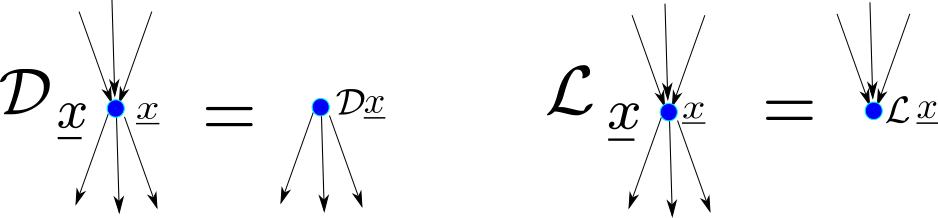
\includegraphics[width=4in]
{do-calc/do-rho-lam.png}
\caption{
The do operator $\cald_\rvx$
converts node $\rvx$
into a root node $\cald \rvx$.
The leaf operator $\call_\rvx$
converts node $\rvx$
into a leaf node $\call\rvx$.
} 
\label{fig-do-rho-lam}
\end{figure}


If
you don't
know yet
what we mean by 
a multi-node
$\rva.$, see
Chapter \ref{ch0-bnet-def}.

Given a bnet
$G$,
we define
as follows
the operators
$\cald_{\rva.}$
and
$\call_{\rva.}$
for a multi-node
$\rva.$.

\beq
\cald_{\rva.}G =
\left[\prod_j \cald_{\rva_j}\right]G
\;,\;\;\;\;
\call_{\rva.}G =
\left[\prod_j \call_{\rva_j}\right]G
\;.
\eeq

Consider a bnet 
whose totality of nodes
is labeled $\rvX.$.
Recall that 

\beq
P(X.)=
\prod_j P(X_j|(X_k)
_{k:\rvX_k\in pa(\rvX_j)})
\;.
\eeq

Define an
operator $\cald$
that acts as follows\footnote{As usual,
$\caln(!x)$ denotes 
a constant 
that is independent of $x$.}: Let
$X.-a.=(X_k)_{k:\rvX_k\notin \rva.}$.

\beqa
P(X.-a.|\cald\rva.=a.)
&=&
\caln(!(X.-a.))
\frac{P(X.)}
{
\prod_{j:\rvX_j\in \rva.}
P(X_j|(X_k)
_{k:\rvX_k\in pa(\rvX_j)})
}
\\
&=&
\caln(!(X.-a.))
\prod_{j:\rvX_j\notin \rva.}
P(X_j|(X_k)
_{k:\rvX_k\in pa(\rvX_j)})
\\
&\neq&
P(X.-a.|\rva.=a.)
\;.
\eeqa
Also,

\beq
P(\cald\rva.=a.)=
\delta(a'., a.)
\;.
\eeq
In words, we replace
the TPM for 
multinode
$\rva.$ by
a delta function.

For instance, for the bnet

\beq
\xymatrix{
\rvr\ar[r]
&\rvx\ar[r]&\rvy
}
\eeq
with 

\beq
P(r, x,y)=P(y|x)P(x|r)P(r)
\;,
\eeq
one has 

\beq
P(r, y|\cald\rvx=x)=P(y|x)P(r)
\eeq
Hence,

\beq
P(y|\cald\rvx=x)=P(y|x)
\eeq


For the bnet

\beq
\xymatrix{
\rvc\ar[d]\ar[rd]
\\
\rvx\ar[r]&\rvy
}
\eeq
with 

\beq
P(x,y, c)=P(y|x, c)P(x|c)P(c)
\;,
\eeq
one has 

\beq
P(y, c|\cald\rvx=x)=P(y|x, c)P(c)
\;.
\eeq
Hence,

\beq
P(y|\cald\rvx=x)=\sum_c P(y|x,c)P(c)
\;.
\eeq
This is called {\bf adjusting the parents
of $\rvx$}.

For
$\rvb.\subset \rvX.-\rva.$,
define

\beq
P(b.|\cald\rva. =a.)=
\sum_{X.-a.-b.}
P(X.-a.|\cald\rva.=a.)
\;,
\eeq
and for
$\rvs.\subset \rvX.-\rva.-\rvb.$,
define

\beq
P(b.|\cald \rva.=a., s.)=
\frac{P(b., s.|\cald\rva.=a.)}
{P(s.|\cald\rva.=a.)}
\;.
\eeq

$P(b.|\cald \rva.=a., s.)$
is denoted by Pearl  by
$P(b.|do(\rva.=a.), s.)$.
I prefer to 
use $\cald$
instead of $do()$.
I will still call $\cald$
a {\bf do operator}.



In $P(y|\cald \rvx=x)$,
node $\rvx$ is turned 
into a root node. This guarantees
that there is
no confounding node
connecting $\rvx$ and
$\rvy$. Such 
confounding nodes 
are unwelcomed 
when calculating
causal effects
between 
the 2 variables $\rvx$ and $\rvy$
 because they 
 introduce 
non-causal
correlations between
the two.
This is also 
what happens
in a {\bf Randomized 
Controlled Trial (RCT)}.
In an RCT
 with treatment $\rvx$,
the value
of $\rvx$ for each patient
is determined by a coin toss,
effectively
turning $\rvx$ into a root node.
Hence, the do operator mimics an RCT.


$P(b.|\cald \rva.=a., s.)$
is said to be {\bf do-identifiable}
(i.e., expressible without do())
if it can be
expressed in terms of
probability distributions
that only
depend on observed 
variables, and that
have no do operators
in them.\footnote{In Statistics,
one says a probability
distribution $P(x;\theta)$
of $x$ that depends on a parameter
$\theta$ is {\bf identifiable}
if  $P(x;\theta_1)=P(x;\theta_2)$
implies $\theta_1=\theta_2$.}

For $\rvx, \rvy\in \bool$,
 the {\bf average causal effect (ACE)}
is defined as

\beq
ACE=
P(y=1|\cald \rvx=1)-
P(y=1|\cald \rvx=0)
\eeq
and the 
{\bf Risk Difference (RD)} 
is defined as

\beq
RD=
P(y=1|\rvx=1)-
P(y=1|\rvx=0)
\;.
\eeq





\section{3 Rules of Do Calculus}
Throughout 
this section, suppose
$\rva., \rvb., \rvr., 
\rvs.$ are disjoint
multinodes in a bnet $G$.


Recall
from Chapter \ref{ch-dsep}
on d-separation,
that  $(\rvb.\perp_G \rva.|\rvr., \rvs.)$
means that 
we have established
from the d-separation
rules that 
that all 
paths in $G$
 from
$\rva.$ to
$\rvb.$
are blocked
if we condition
on $\rvr.\cup \rvs.$.
Recall also that:

\begin{itemize}[\;]
\item {\bf Rule 0:} Insertion or
 deletion of
 observations, without
do operators.

\rulezeroif
\begin{itemize}[$\checkmark$]

\item $\rulezeroP$
\quad(i.e., \rulezerothen)
\\
$\rulezeropic$
\item $\rulezeroH$
\end{itemize}

\end{itemize}
Zeroing an arrow is the same as deleting it.
The 3 rules of Do Calculus
can be presented in the same
format. 


\begin{itemize}
\item {\bf Rule 1:} 
Insertion or deletion of
 observations 

\ruleoneif
\begin{itemize}[$\checkmark$]

\item $\ruleoneP$
\quad(i.e., \ruleonethen)
\\
$\ruleonepic$
\item $\ruleoneH$
\end{itemize}


\item {\bf Rule 2:} Action or 
observation exchange 

\ruletwoif
\begin{itemize}[$\checkmark$]
\item $\ruletwoP$
\quad(i.e., \ruletwothen)
\\
$\ruletwopicA$
\\
$\ruletwopicB$
\\
In this rule, the node
is split into a $\cald\rva.=a.$ node
and a $a.$
node. The original 
node keeps the arrows,
 and the new node is a root node.

\item $\ruletwoH$
\end{itemize}

\item {\bf Rule 3:} Insertion and
 deletion of actions


\rulethreeif
\begin{itemize}[$\checkmark$]

\item $\rulethreeP$
\quad(i.e., \rulethreethen)
\\
$\rulethreepic$
\item $\rulethreeH$
\end{itemize}


\end{itemize}

\begin{figure}[h!]
\centering
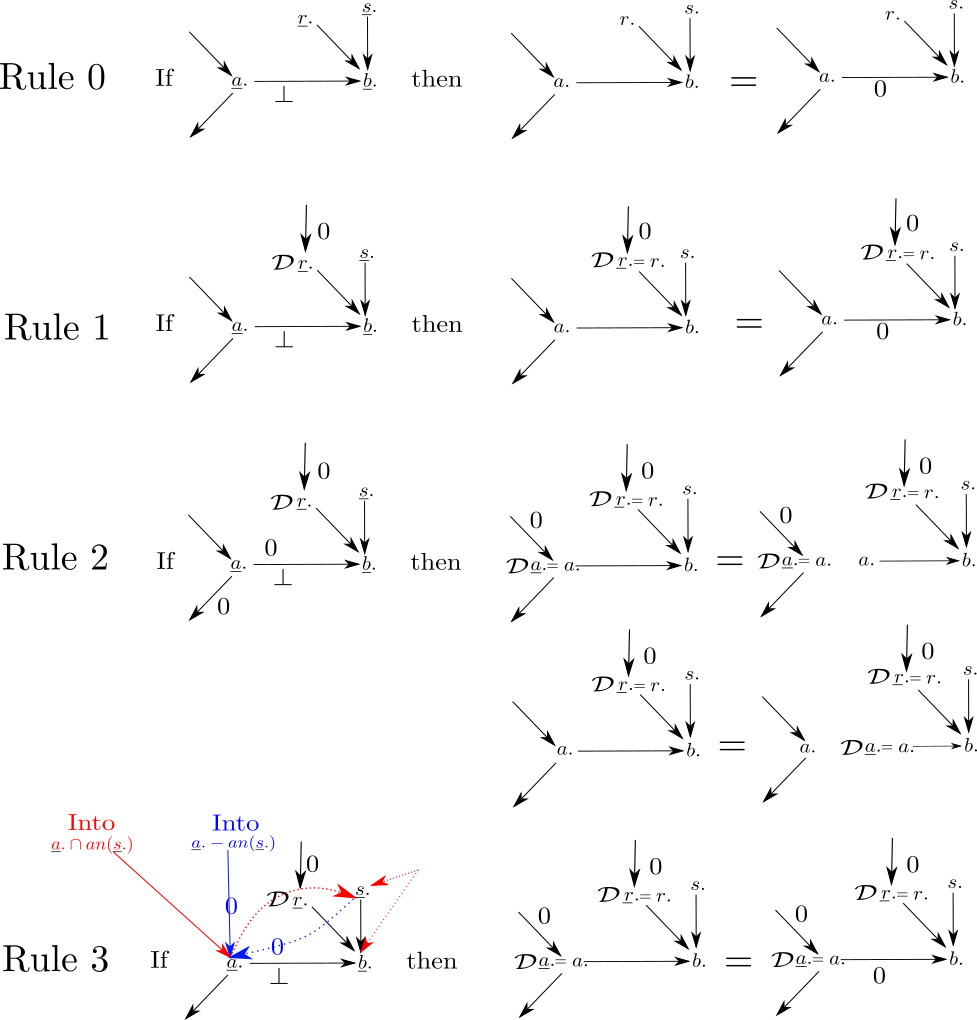
\includegraphics[width=5in]
{do-calc/do-rules.png}
\caption{Pictorial representation of the
 rules of Do Calculus. $an(\rvs.)$
stands for the ancestors 
of $\rvs.$.
In Rule 2, we zero the arrows
leaving $\rva.$
and ascertain that 
there is no flow of info 
between $\rva.$ and $\rvb.$
under those circumstances.
In Rule 3, 
as shown by
the dotted arrows, conditioning
on $\rvs.$
is enough to block 
paths going from $\rvb.$
into
$\color{blue}\rva.-an(\rvs.)$,
but it is not sufficient to block 
paths going from $\rvb.$
into
$\color{red}\rva.\cap an(\rvs.)$.
In the example with red dotted
arrows,
conditioning
on $\rvs.$
opens a path
between $\rva.$ and $\rvb.$
in which $\rvs.$
is a collider.
That is the reason for 
zeroing arrows going into 
$\color{blue}\rva.-an(\rvs.)$,
but not zeroing arrows 
going into
$\color{red}\rva.\cap an(\rvs.)$.
} 
\label{fig-do-rules}
\end{figure}

See Fig.\ref{fig-do-rules}
for a pictorial representation of these
 rules.

These rules have been
proven to be 
sufficient
for removing
all do operators
from an expression
for 
which it 
is possible to do so.

Next we discuss
two formulae that can be
proven using
Do Calculus:
the backdoor and the
frontdoor
adjustment formulae.

The 
backdoor formula
adjusts one multinode
and the 
frontdoor formula adjusts two.

\section{Parent Adjustment Formula}


Suppose 
that $\rvx., \rvy., \rvz.$
are disjoint multinodes
and their union equals
 the
totality of all nodes of
a bnet. 
Suppose we have data
available that allows us  to
estimate $P(x., y., z.)$.
Hence, all nodes of the bnet
are observable.
Furthermore,
suppose $\rvz.=pa(\rvx.)$.
In other words,
we are 
considering the bnet

\beq
\xymatrix{
\rvz.\ar[d]\ar[dr]
\\
\rvx.\ar[r]&\rvy.
}
\;.
\eeq

Then

\beq
P(y., z.|\cald \rvx.=x.)
=P(y.|x., z.)P(z.)
\eeq
so

\beq
P(y.|\cald \rvx.=x.)
=\sum_{z.}P(y.|x., z.)P(z.)
\;.
\eeq
This is called
{\bf adjusting the parents}
of $\rvx.$.


We say that 
we are {\bf adjusting 
or controlling a node $\rva$}
if we condition 
a probability on $\rva$ and 
then we average 
that probability over $\rva$.
More generally, 
we can adjust a whole
multinode $\rva.$ together.

Next,
we will introduce 
a generalization
of 
this parent adjustment formula
called the 
backdoor adjustment formula.
In a backdoor adjustment formula,
the adjusted multinode
is not necessarily
 the parents of $\rvx.$.

\section{Backdoor Adjustment Formula}

See Chapter \ref{ch-bdoor}
for examples of the use of the 
backdoor adjustment formula.
In this section,
we shall mainly be
concerned with
proving this
theorem
using Do Calculus.

For any two
disjoint
multinodes $\rvx.$
and $\rvy.$,
we define a {\bf backdoor path}
from $\rvx.$ to $\rvy.$
as a path from $\rvx.$
and $\rvy.$ that
starts with an arrow pointing into 
$\rvx.$,

\bdoordef

{\bf Motivation for BD criterion}: 
Part 1 rules out
paths 
from $\rvx$
to $\rvy$
containing a fork node (confounder)
which, if not blocked by conditioning on $\rvz.$, 
 would introduce a
non-causal correlation 
(confounder bias).
Part 2 rules out
a directed path
from $\rvx$ to $\rvy$
that has a mediator node
blocked by conditioning on $\rvz.$
or a collider node
unblocked by conditioning on $\rvz.$.



\begin{claim} (Backdoor 
Adjustment Formula)

\bdoorclaim
\end{claim}
\proof

For simplicity,
let us omit
the dots from the
multinodes.
If
$z$
satisfies the
backdoor
criterion
relative
to
$(\rvx, \rvy)$,
then
$\rvx, \rvy, \rvz$
might
have the following 
structure.


\beq
\xymatrix{
{\rvz}\ar[d]\ar[rd]
\ar@{<-->}@/_1pc/[d]
&*++[F-o]{\rvu}\ar[d]
&*++[F-o]{\rvv}
\\
\rvx\ar[r]\ar[ur]\ar[rru]
&\rvy\ar[ru]
}
\label{eq-bdoor-special}
\eeq

See Claim \ref{cl-decBackDoor}
for a proof of this claim
for the
special case Eq.(\ref{eq-bdoor-special}).
\qed

Note that the backdoor adjustment  formula
can be written as
 
\beqa
P(y.|\cald \rvx. =x.)
&=&
\sum_{z.}P(y.|x., z.)P(z.)
\\
&=&
\sum_{z.}\frac{P(y.,x., z.)}
{P(x.|z.)}
\eeqa
This assumes $P(x.|z.)\neq 0$
for all $x., z.$. This assumption
is referred to
as {\bf positivity},
and is violated
if $P(x.|z.)=\delta(x., x.(z.))$.
$P(x.|z.)$ is called the 
{\bf propensity score}
of $x.$ given $z.$.
This
equation does 
{\bf inverse probability weighting}.
One
can approximate $P(x.|z.)$ 
in this equation
to get
an approximation
to  $P(y|\cald\rvx=x)$.


\section{Frontdoor Adjustment Formula}
See Chapter \ref{ch-fdoor}
for examples of the use of the 
frontdoor adjustment formula.
In this section,
we shall mainly be
concerned with
proving this
theorem
using Do Calculus.

\fdoordef

\begin{claim} (Frontdoor Adjustment
Formula)

\fdoorclaim

\end{claim}
\proof


For simplicity,
let us omit
the dots from the
multinodes.
If
$\rvm$
satisfies the
frontdoor
criterion
relative
to
$(\rvx, \rvy)$,
then
$\rvx, \rvm, \rvy$
might 
have the following 
structure,
where node $\rvc$
is unobserved.


\beq
\xymatrix{
&*++[F-o]{\rvc}\ar[ld]\ar[rd]
\\
\rvx\ar[r]&\rvm\ar[r]&\rvy
}
\label{eq-fdoor-special}
\eeq

See Claim \ref{cl-decFrontDoor}
for a proof of this claim
for the special case 
Eq.(\ref{eq-fdoor-special}).


See also Ref.\cite{pearl-frontdoor}
for a proof by Pearl
of the Frontdoor Adjustment Formula
without 
using Do Calculus.
\qed

\section{Comparison
of Backdoor and Frontdoor
adjustment formulae}

Define a {\bf direct effect path}
for a query $P(y|\cald\rvx=x,z.)$
as a directed path that starts at $\rvx$
and ends
at $\rvy$. A backdoor path 
(i.e., one that connects
$\rvx$ and $\rvy$ starting
with an arrow
pointing into $\rvx$),
is not a direct effect path;
it's an {\bf indirect effect path}.

Note that in the backdoor AF (adjustment
formula), we can find a possibly empty
observed multinode
$\rvz.$ such that if
we condition
on $\rvz.$,
all indirect effect paths are blocked.
In the frontdoor AF,
we can't find a multinode $\rvz.$
that blocks all indirect effect
paths. 
Despite this,
in the frontdoor scenario,
the do-query is
identifiable and
an adjustment formula
exists. 
How is that possible?
The frontdoor AF 
uses the backdoor AF once
and then it uses 
the backdoor AF again,
a second time, on 
the result of the first use.
The frontdoor AF 
replaces a
sum over an unobserved node
by a sum over an observed one.



\section{Do operator for DEN diagrams}

Recall that
the structural
equations
for a linear DEN, as
given
by Eq.(\ref{eq-mat-fully-conn})
of Chapter \ref{ch-linear-sys}, are:

\beq
\rvx=A\rvx +\rvu
\;.
\label{eq-struc-pre-rho}
\eeq
Therefore,

\beq
\rvx=(1-A)^{-1}\rvu
\eeq
which
can be 
represented for
both linear
and non-linear DEN
diagrams by:

\beq
\rvx_i = x_i(\rvu.)
\eeq 

If now
we apply the
operator
$\cald_{\rva=a}$
to 
the diagram
described by
the structural
equations Eqs.\ref{eq-struc-pre-rho},
we get the following
new
structural
equations:

\beq
\rvx^*_i =\left\{
\begin{array}{lll}
 \sum_{j<i} A_{i|j}\rvx^*_j + \rvu_i&
 \text{if $\rvx_i\neq \rva$}
\\
a&
\text{if $\rvx_i=\rva$}
\end{array}
\right.
\label{eq-ith-struc-post-rho}
\;,
\eeq
where we are
calling 
$\rvx^*_i$ the
nodes
of the DEN 
diagram post intervention.

Eqs.(\ref{eq-ith-struc-post-rho})
can be expressed in matrix notation
as follows.
Define $\pi_\rva$ to
be the $nx\times nx$ matrix 
with all entries equal
to  zero
except for the $(i_0,i_0)$ entry, which is 1.
And define $e_\rva$
to be the column vector
with all entries zero
except for the $i_0$'th one, 
which is 1. 
Here
$i_0$  
is
defined so that $\rvx_{i_0}=\rva$.
In other words, $\pi_\rva$ and $e_\rva$
are defined by

\beq
(\pi_\rva)_{i,j}= \indi(i=j, \rva=\rvx_i)
\;
\eeq
and

\beq
(e_\rva)_i=\indi(\rva=\rvx_i)
\;,
\eeq
for $i, j\in \{0, 1, \ldots, nx-1\}$.
Next define

\beq
\pi_{!\rva}=1-\pi_\rva
\;,
\eeq

\beq
A^*=\pi_{!\rva} A
\;,
\eeq
and

\beq
\rvu_{!\rva}=\pi_{!\rva} \rvu
\;.
\eeq
The effect
of pre-multiplying
the matrix
$A$ 
and the column vector $\rvu$ by
$\pi_{!\rva}$
is to leave all rows
intact except for
the $i_0$
row, which is set to zero. Here
 $i_0$ is defined by
 $\rva=\rvx_{i_0}$.
Finally,
using 
all
of the
variables just defined,
we can express the
structural equations
of the linear DEN diagram,
post intervention, as


\beq
\rvx^*= A^* \rvx^* + \rvu_{!\rva} +
ae_\rva
\;.
\eeq
Thus,

\beq
\rvx^*=(1-A^*)^{-1} (\rvu_{!\rva}+ae_\rva)
\;.
\eeq
which
can be 
represented for
both linear
and non-linear DEN
diagrams by:

\beq
\rvx^*_i=x^*_i(\rvu_{!\rva},a)
\;.
\eeq



For any bnet,

\beq
P(\rvy=y|\rvx=x)
=
P_{G}(\rvy=y|\rvx=x)
\eeq

\beq
P(\rvy=y|\cald\rvx=x)
=
P_{\cald_{\rvx=x}G}(\rvy=y)
\eeq


\begin{claim}
For a non-linear DEN diagram,



\beq
P(y|\cald\rvx=x)=
E\left[
\delta[y, y(\rvu_{!\rvx},x)]\right]
\;.
\eeq
\end{claim}
\proof
\beqa
P(\rvy=y|\cald\rvx=x)
&=&
P_{\cald_{\rvx=x}G}(\rvy=y)
\\
&=&\sum_{u_{!\rvx}}P(u_{!\rvx})
P_{\cald_{\rvx=x}G}
(\rvy=y|u_{!\rvx})
\\
&=&\sum_{u_{!\rvx}}P(u_{!\rvx})
\delta[y, y(u_{!\rvx},x)]
\\
&=&
E_{\rvu_{!\rvx}}
[\delta[y, y(u_{!\rvx}, x)]]
\\
&=&
E[\delta[y,y(\rvu_{!\rvx}, x)]]
\eeqa
\qed

\begin{claim}
For a nonlinear DEN diagram,

\beq
E[\rvy|\cald \rvx=x]=
E[y(\rvu_{!\rvx}, x)]
\;.
\eeq
\end{claim}
\proof

\beqa
E[\rvy|\cald \rvx=x]
&=&
\sum_{y}
yP(\rvy=y|\cald\rvx=x)
\\
&=&
\sum_{y}
yE[
\delta[y, y(u_{!\rvx},x)]]
\\
&=&
E[y(\rvu_{!\rvx}, x)]
\eeqa
\qed


For any bnet
\beqa
P(y|\cald\rvx=x, z)&=&
\frac{P(y, z|\cald\rvx=x)}
{P(z|\cald\rvx=x)}
=
P_{\cald_{\rvx=x}G}(y|x, z)
\eeqa

For a nonlinear DEN diagram,
\beq
P(y, z|\cald\rvx=x)
=
\sum_{u_{!\rvx}}P(u_{!\rvx})
\delta[y, y(u_{!\rvx},x)]
\delta[z, z(u_{!\rvx},x)]
\eeq

\beq
P(z|\cald\rvx=x)=
\sum_{u_{!\rvx}}P(u_{!\rvx})
\delta[z, z(u_{!\rvx},x)]
\;.
\eeq
